\ProvidesFile{questions.tex}[Questions]
\section{Questions (Вопросы)}
\subsection{Общие вопросы}
Начинаются со вспомогательных слов\\
\sample{Do you smoke?}\\
\sample{Yes, I do}\\
\sample{No, I don't}

\subsection{Специальные вопросы}
\p
Начинаются с вопросительного слова + вспомогательное\\
\sample{Who gave you this?}\\
\bld{*} После \bld{who} в \bld{Past Simple} и \bld{Present Simple}
вспомогательное слово не используется. Вместо него используем глагол в нужной форме.\\
\sample{Who gives you money?}\\
\sample{Who told you that?}\\
\sample{Who is helping you now?}\\
\sample{Whose car is this?}

\subsection{Вопросы с предлогом}
\[\fbox{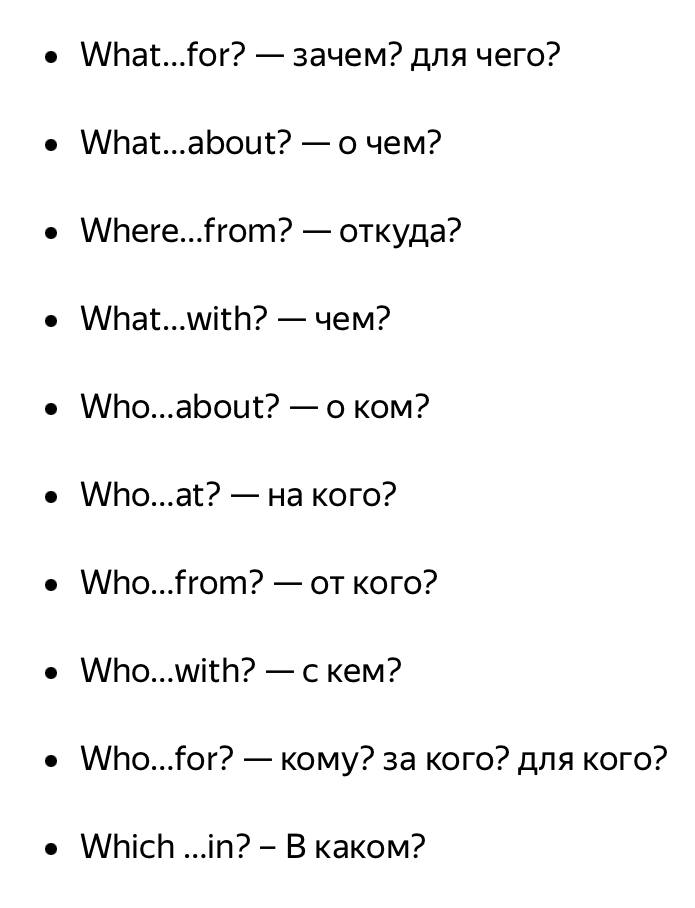
\includegraphics[width=0.5\textwidth]{img/questions_prepositions.jpg}}\]
\sample{What are you doing it for?}\\
\sample{What are you speaking about?}\\
\sample{What did you cut it with?}

\subsection{Tag questions}
\p
Вопросы, у которых в конце:
\begin{enumerate}
    \item \bld{Да?}
    \item \bld{Не так ли?}
    \item \bld{Правда?}
    \item \bld{Не правда ли?}
\end{enumerate}
В английском языке хвостик зависит от времени главной части.\\
Хвостик всегда противоположный и всегда заканчивается на первое слово главной части (либо же на соответствующее
местоимение, если имя собственное)\\
Главная часть всегда + или - (не?)\\
\sample{They live near here, don't they?}\\
\sample{There was a lot of noise, wasn't there?}\\
\sample{Tom won't be late, will he?}\\\\
\bld{Исключения}
\begin{enumerate}
    \item Для \bld{I} мы используем \bld{aren't I}
    \item Для \bld{повелительного наклонения} мы используется \bld{will you?\textbackslash won't you?}
    \item Для \bld{let's} используем \bld{shall we?}
\end{enumerate}
\sample{I am your teacher, aren't I?}

\subsection{Удивления}
\p
Это те же хвостики, но без смены знака. Хвостик говорит наш собеседник. Исключений нет\\
\sample{--I have bought a new car}\\
\sample{--Have you?}

\subsection{Я тоже}
\p
Стандартные способы выразить согласие\\
\sample{I like apples}\\
\sample{Me too}\\\\
\sample{I don't like apples}\\
\sample{Me either}\\\\
Ещё способ выразить согласие\textbackslash несогласие\\
\sample{I don't like apples}\\
\sample{+ So do I}\\
\sample{-- Neither do I}
